\setchapterpreamble[u]{\margintoc}
\chapter{Optimizing modular structures}
Introduction
\todo{change $N_T$ con $N_\text{T}$ }
\section{Formulation of a modular structure optimization algorithm}
why cellular, which are the advantages

intro there are different type of approach that we could use, full scale and multiscale

intro multiscale.

numerical homogenization

intro full scale

the problem on the number of subsections needed to correctly foresee the mechanical behaviour
\subsection{Variable linking}
we link different domains toghether

math formulation used, talk already about the possibility to use diffeernt cells

$\bar{n}$ is the number of candidate bars of one cell. Iterator $i$

\todo{image with i,j,t}

$\vect{a} = \sum_{t=1}^{N_T} \vect{g}_t\otimes\bar{\vect{a}}_t = \sum_{t=1}^{N_T} \begin{bmatrix}
    g_{1,t} \: \bar{\vect{a}}_t \\
    \vdots\\
    g_{N_{\text{sub}},t} \: \bar{\vect{a}}_t 
    \end{bmatrix}$

$\matr{G} \in \mathbb{B}^{N_{\text{sub}},N_T} $
where $\mathbb{B}=\lbrace 0,1 \rbrace$ is Boolean domain.

$g_{j,t} =
\begin{cases}
  1 & \text{if subdomain $j$ is of type $t$,} \\
  0 & \text{otherwise.} 
\end{cases}$

Make a simple example to show how the matrix G vary for different examples. we are here considering only nt=1, so G is a vector, but the notation is important

$\matr{G}=
\begin{bmatrix} 
    1 & 0 \\
    1 & 0 \\
    1 & 0 \\
    0 & 1 \\
    0 & 1 \\
    0 & 1 \\
\end{bmatrix}.$

number of design variables is low, buth still high constraints

mini investigation on the fact that 
\subsection{Topological buckling of modular structures}
Explain only how the constraint is handled now that the cells are multiple $\bar{a}_{r}\geq \bar{a}_{r=1} \quad r \in \mathcal{C}_{l,r}(\bar{\vect{a}})$

\section{Optimization formulation}

We concentrate on the simplest type, with $N_T=1$

the formulation $\mathbb{P}_\text{1,m}$ is stated in terms of members' cross-sectional area $\vect{a}$, member forces $\vect{q}$ and nodal displacements $\vect{U}$ as follows:
\begin{equation}
    \begin{aligned}
    \min_{\bar{\vect{a}}, \vect{q}, \vect{U}}   && V &= \vect{\ell}^{T}\vect{a}\\
    \textrm{s.t.}  && \vect{a} &= \matr{G}\otimes\bar{\vect{a}} \\ 
    && \matr{B}\vect{q} &= \vect{f} && \\
    && \vect{q} &= \frac{\vect{a}E}{\vect{\ell}}\vect{b}^T\vect{U} &&  \\
    && \vect{q} &\geq -\frac{s\vect{a}^2}{\vect{\ell}^{*2}} &&  \\
    && -\sigma_c\vect{a} &\leq \vect{q} \leq \sigma_t\vect{a} &&  \\
    && \bar{a}_{r}&\geq \bar{a}_{r=1} && r \in \mathcal{C}_{l,r}(\bar{\vect{a}}) \\
    && \bar{\vect{a}} &\geq 0. \\
    \end{aligned}
    \tag{$\mathbb{P}_\text{1,m}$}
    \label{eq:optim_complete}
\end{equation}

$N_{\text{sub}}$
${\bar{\vect{a}}} \in \mathbb{R}_+^{N_T \cdot \bar{n}} $ where $N_T$
${\vect{a}} :=  \{\vect{a}^j \;|\; \forall j \in [1,\dots,N_{\text{sub}}]\}$
${\bar{\vect{a}}} :=  \{ \bar{\vect{a}}_t \;|\; \forall t \in [1,\dots,N_T]\}$ represent the vector of the cross-sectional areas of the cells
$\bar{n}$ is the number of candidate bars of one cell.

\subsection{Sensitivity analysis}
how the sensitivity is changed with respect to the variable linking

just a sum more to do for constraints

\todo{image for sensitivity ?}
\section{Numerical application}
\todo{find some litterature case that we can use to compare at least visually, maybe the sandwich structure that joseph suggested me}
\subsection{On the equivalence of multi load cases and modular structures}
\begin{figure}[]
    \hspace*{\fill}
    \subcaptionbox{}{\includegraphics[height=3cm]{figures/05_cellular_opt/00_cell_multi_eq_bcs/cell_bcs.pdf}}
    \hfill
    \subcaptionbox{}{\includegraphics[height=3cm]{figures/05_cellular_opt/00_cell_multi_eq_bcs/multiload_bcs.pdf}}
    \hspace*{\fill}
    \caption{}
    \label{fig:05_cell_multi_eq_bcs}
\end{figure}

\begin{figure}[]
    \hspace*{\fill}
    \subcaptionbox{}{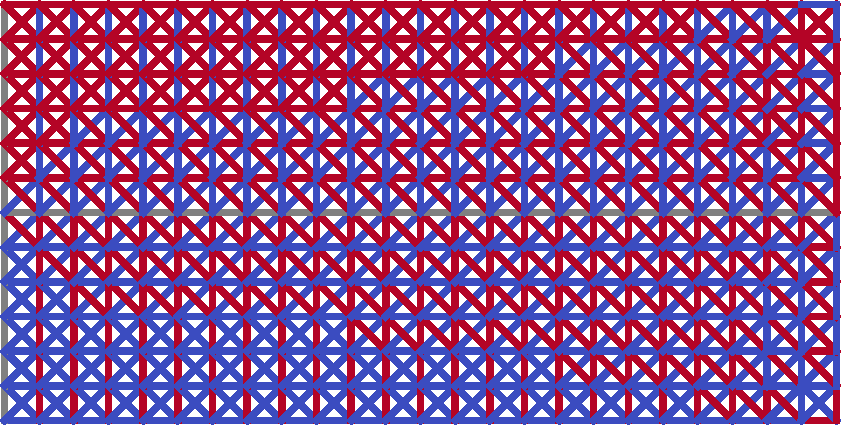
\includegraphics[height=3cm]{figures/05_cellular_opt/00_cell_multi_equivalence/cell.pdf}}
    \hfill
    \subcaptionbox{}{\includegraphics[height=3cm]{figures/05_cellular_opt/00_cell_multi_equivalence/multiload.pdf}}
    \hspace*{\fill}
    \caption{}
    \label{fig:05_cell_multi_eq}
\end{figure}
\subsection{Parametric study on the number, the shape, and the complexity of the module}

\todo{use blender to generate images}

\todo{check always the number of design variables, constraints and time}

\todo{different tables for every parametric study with iteration count}
Simply supported 3D beam

\subsection{Comparison with the optimized octet truss}


\section{Conclusion}